\documentclass[letterpaper,11pt]{article}
\usepackage{graphicx}
\usepackage{listings}
\usepackage[super]{nth}
\usepackage[hyphens]{url}
\usepackage{amsmath}
\usepackage[makeroom]{cancel}
\usepackage[table]{xcolor}
\usepackage{comment}
\usepackage[space]{grffile}

\lstset{
	basicstyle=\footnotesize,
	breaklines=true,
}

\begin{document}

\begin{titlepage}

\begin{center}

\Huge{Assignment 6}

\Large{CS 595:  Introduction to Web Science}

\Large{Fall 2013}

\Large{Shawn M. Jones}

\Large Finished on \today

\end{center}

\end{titlepage}

\newpage
\section*{1}

\subsection*{Question}

\begingroup
\fontsize{6pt}{10pt}\selectfont
\begin{verbatim}
1.  We know the result of the Karate Club (Zachary, 1977) split.
Prove or disprove that the result of split could have been predicted
by the weighted graph of social interactions.  How well does the
mathematical model represent reality?

Generously document your answer with all supporting equations, code,
graphs, arguments, etc.

Useful sources include:

* Original paper

http://aris.ss.uci.edu/~lin/76.pdf

* Slides

http://www-personal.umich.edu/~ladamic/courses/networks/si614w06/ppt/lecture18.ppt

http://clair.si.umich.edu/si767/papers/Week03/Community/CommunityDetection.pptx

* Code and data

http://networkx.github.io/documentation/latest/examples/graph/karate_club.html

http://nbviewer.ipython.org/url/courses.cit.cornell.edu/info6010/resources/11notes.ipynb

http://stackoverflow.com/questions/9471906/what-are-the-differences-between-community-detection-algorithms-in-igraph/9478989#9478989

http://stackoverflow.com/questions/5822265/are-there-implementations-of-algorithms-for-community-detection-in-graphs

http://konect.uni-koblenz.de/networks/ucidata-zachary

http://vlado.fmf.uni-lj.si/pub/networks/data/ucinet/ucidata.htm#zachary
\end{verbatim}
\endgroup

\newpage
\subsection*{Answer}

The results of the Karate Club split could have been predicted using the weighted graph of social interactions.  The level of accuracy depends on the algorithm used.

The weighted graph of Karate Club data was loaded into R and run through the program shown in Listing \ref{lst:q1codeR}.  Lines $24$-$44$ use the hierarchical divisive Girvan-Newman Betweenness Clustering algorithm to split the graph, stopping when two clusters are created.  From this code, the graphs in Figures \ref{fig:club-before} and \ref{fig:club-after} were produced.

Using this implementation, we can create a split in the group, and even predict that there will be a split.  The algorithm goes through 18 iterations before two groups are created.

Figure \ref{fig:club-before} shows the graph of the Karate Club's relationships prior to the split.  As with Zachary's original paper, the node labeled $34$ represents ``John A.'' and the node labeled $1$ represents ``Mr. Hi''.

Figure \ref{fig:club-after} shows the graph of the Karate Club's relationships after running the Girvan-Newman Betweenness Clustering Algorithm from Listing \ref{lst:q1codeR}.

Table \ref{tab:results} shows the individual identifiers in column 1.  Column 2 shows the actual recorded group membership after the split (\emph{Officers'} is John A's faction).  Column 3 shows Zachary's modeled group membership after the split.  Column 4 shows my Girvan-Newman modeled group membership after the split.  Column 5 shows whether my Girvan-Newman implementation resulted in a \emph{Hit} (correctly calculated membership) or \emph{Miss} (incorrectly calculated membership).

Zachary's Ford and Fulkerson procedure had a $97\%$ success rate.  My Girvan-Newman implementation has a $94\%$ success rate, making it inferior in this case but still effective at predicting almost all of the group memberships.  My implementation also predicted that individual $9$ would stay with Mr. Hi, which is the one membership that Zachary missed.

Either way, it can be shown that this split could have been predicted to greater than $90\%$ accuracy using this data.

One item that Zachary's paper did not take into account was when this split could have been predicted.  A possibility for future research is to build snapshot graphs for a given group \emph{over time}, and then using the Ford and Fulkerson procedure or the Girvan-Newman algorithm to find the earliest point at which a split can be predicted.  Is it possible that the split could have been accurately predicted when one or more of the edge weights was lower (e.g. an individual hadn't attended a karate tournament \emph{yet}, but will gain an edge point for doing so in a subsequent snapshot graph)?

\clearpage
\begin{table}
\small
\begin{tabular}{ | c | p{2cm} | p{2cm} | p{2cm} | p{2cm} | }
\hline
Individual & Actual Group\newline Membership From Split & Zachary's Ford and Fulkerson Procedure Modeled Group\newline Membership From Split & Girvan-Newman Modeled Group\newline Membership From Split & Hit/Miss For Girvan-Newman\\
\hline
1 & Mr. Hi & Mr. Hi & Mr. Hi & Hit \\
\hline
2 & Mr. Hi & Mr. Hi & Mr. Hi & Hit \\
\hline
3 & Mr. Hi & Mr. Hi & Mr. Hi & Hit \\
\hline
4 & Mr. Hi & Mr. Hi & Mr. Hi & Hit \\
\hline
5 & Mr. Hi & Mr. Hi & Mr. Hi & Hit \\
\hline
6 & Mr. Hi & Mr. Hi & Mr. Hi & Hit \\
\hline
7 & Mr. Hi & Mr. Hi & Mr. Hi & Hit \\
\hline
8 & Mr. Hi & Mr. Hi & Mr. Hi & Hit \\
\hline
9 & Mr. Hi & Officers' & Mr. Hi & Hit \\
\hline
10 & Officers' & Officers' & Mr. Hi & Miss \\
\hline
11 & Mr. Hi & Mr. Hi & Mr. Hi & Hit \\
\hline
12 & Mr. Hi & Mr. Hi & Mr. Hi & Hit \\
\hline
13 & Mr. Hi & Mr. Hi & Mr. Hi & Hit \\
\hline
14 & Mr. Hi & Mr. Hi & Mr. Hi & Hit \\
\hline
15 & Officers' & Officers' & Officers' & Hit \\
\hline
16 & Officers' & Officers' & Officers' & Hit \\
\hline
17 & Mr. Hi & Mr. Hi & Mr. Hi & Hit \\
\hline
18 & Mr. Hi & Mr. Hi & Mr. Hi & Hit \\
\hline
19 & Officers' & Officers' & Officers' & Hit \\
\hline
20 & Mr. Hi & Mr. Hi & Mr. Hi & Hit \\
\hline
21 & Officers' & Officers' & Officers' & Hit \\
\hline
22 & Mr. Hi & Mr. Hi & Mr. Hi & Hit \\
\hline
23 & Officers' & Officers' & Officers' & Hit \\
\hline
24 & Officers' & Officers' & Officers' & Hit \\
\hline
25 & Officers' & Officers' & Officers' & Hit \\
\hline
26 & Officers' & Officers' & Officers' & Hit \\
\hline
27 & Officers' & Officers' & Officers' & Hit \\
\hline
28 & Officers' & Officers' & Officers' & Hit \\
\hline
29 & Officers' & Officers' & Officers' & Hit \\
\hline
30 & Officers' & Officers' & Officers' & Hit \\
\hline
31 & Officers' & Officers' & Officers' & Hit \\
\hline
32 & Officers' & Officers' & Mr. Hi & Miss \\
\hline
33 & Officers' & Officers' & Officers' & Hit \\
\hline
34 & Officers' & Officers' & Officers' & Hit \\
\hline
\end{tabular}
\caption{Results of Split, as predicted by Girvan-Newman Implementation}
\label{tab:results}
\end{table}

\clearpage
\begin{figure}[h]
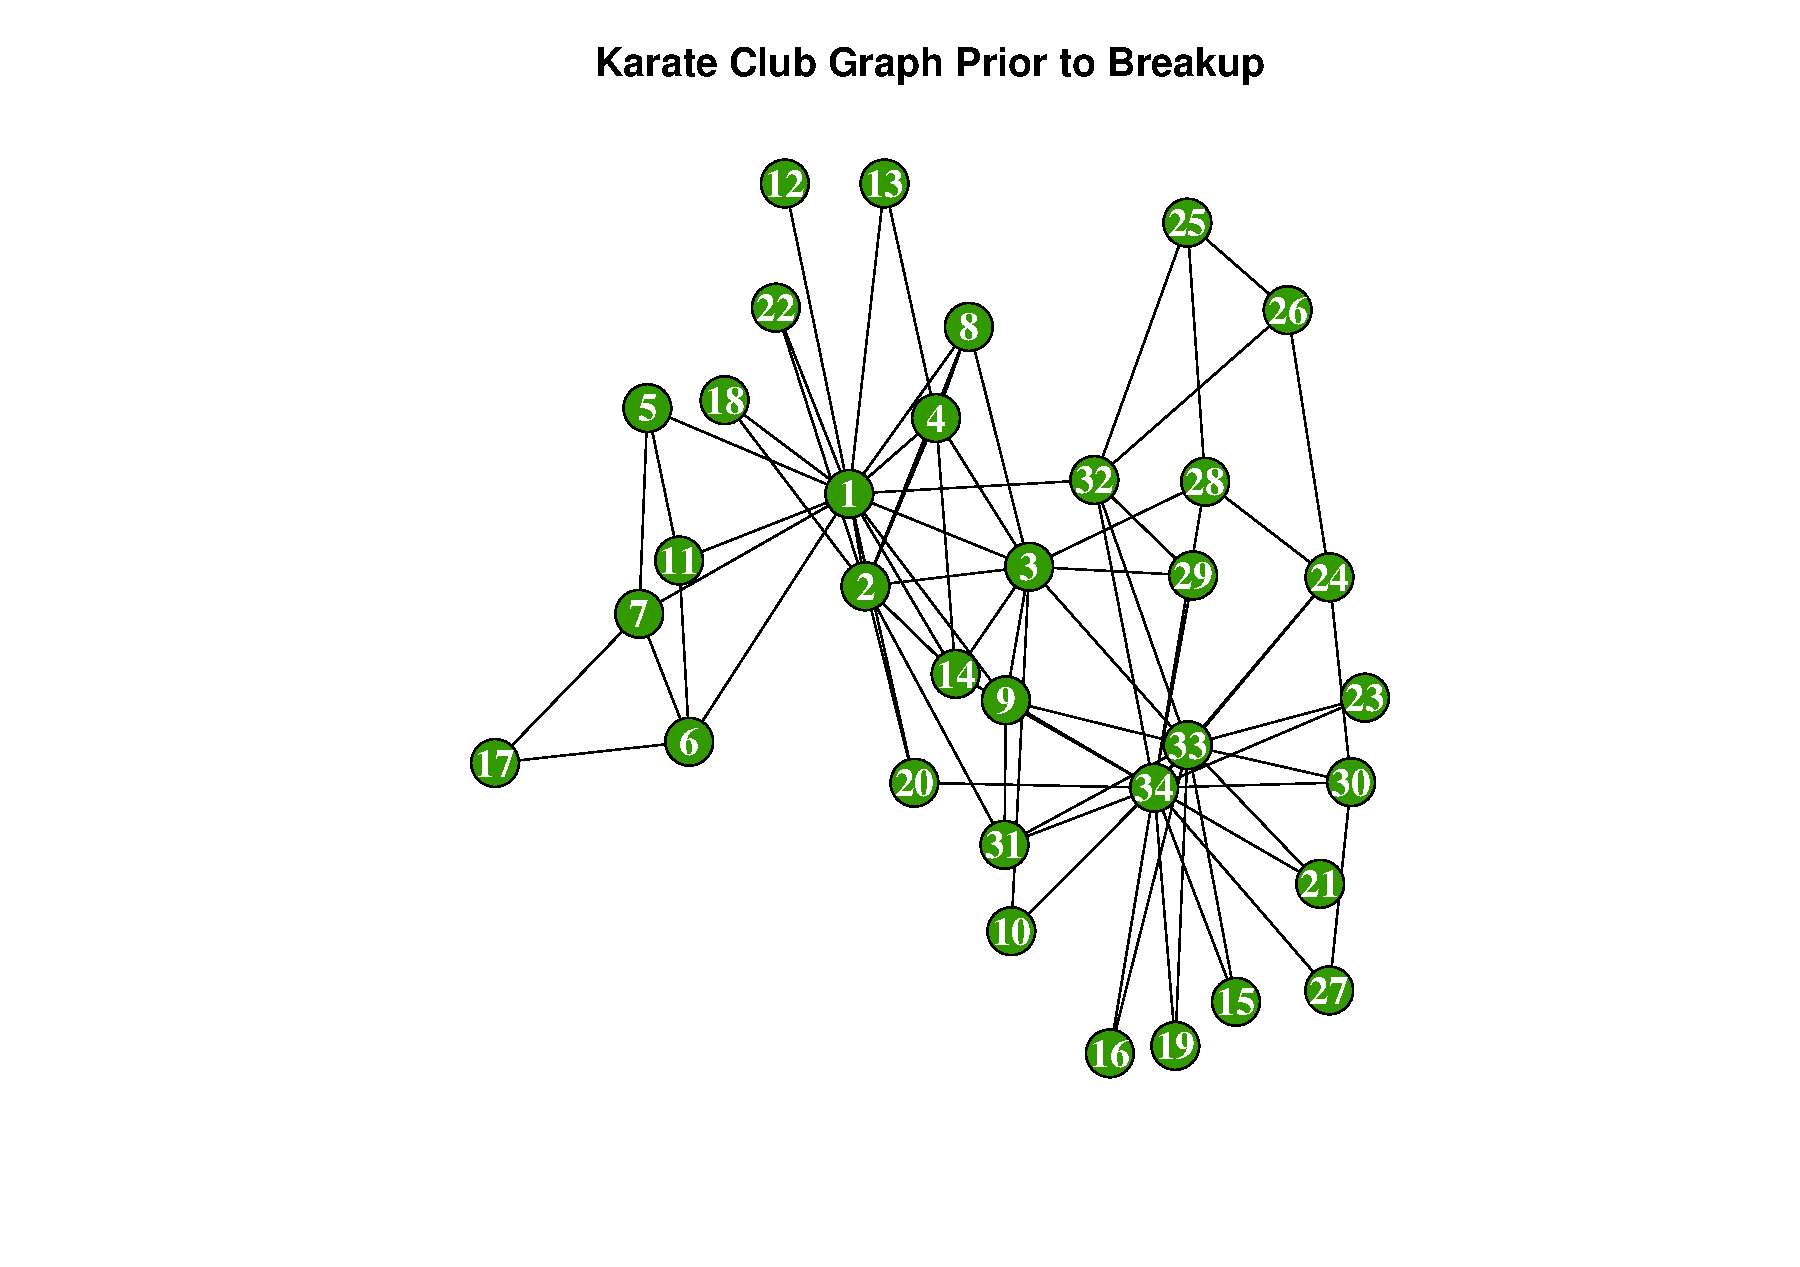
\includegraphics[scale=0.5]{club-before.pdf}
\caption{Karate Club Graph Before Split}
\label{fig:club-before}
\end{figure}

\clearpage
\begin{figure}[h]
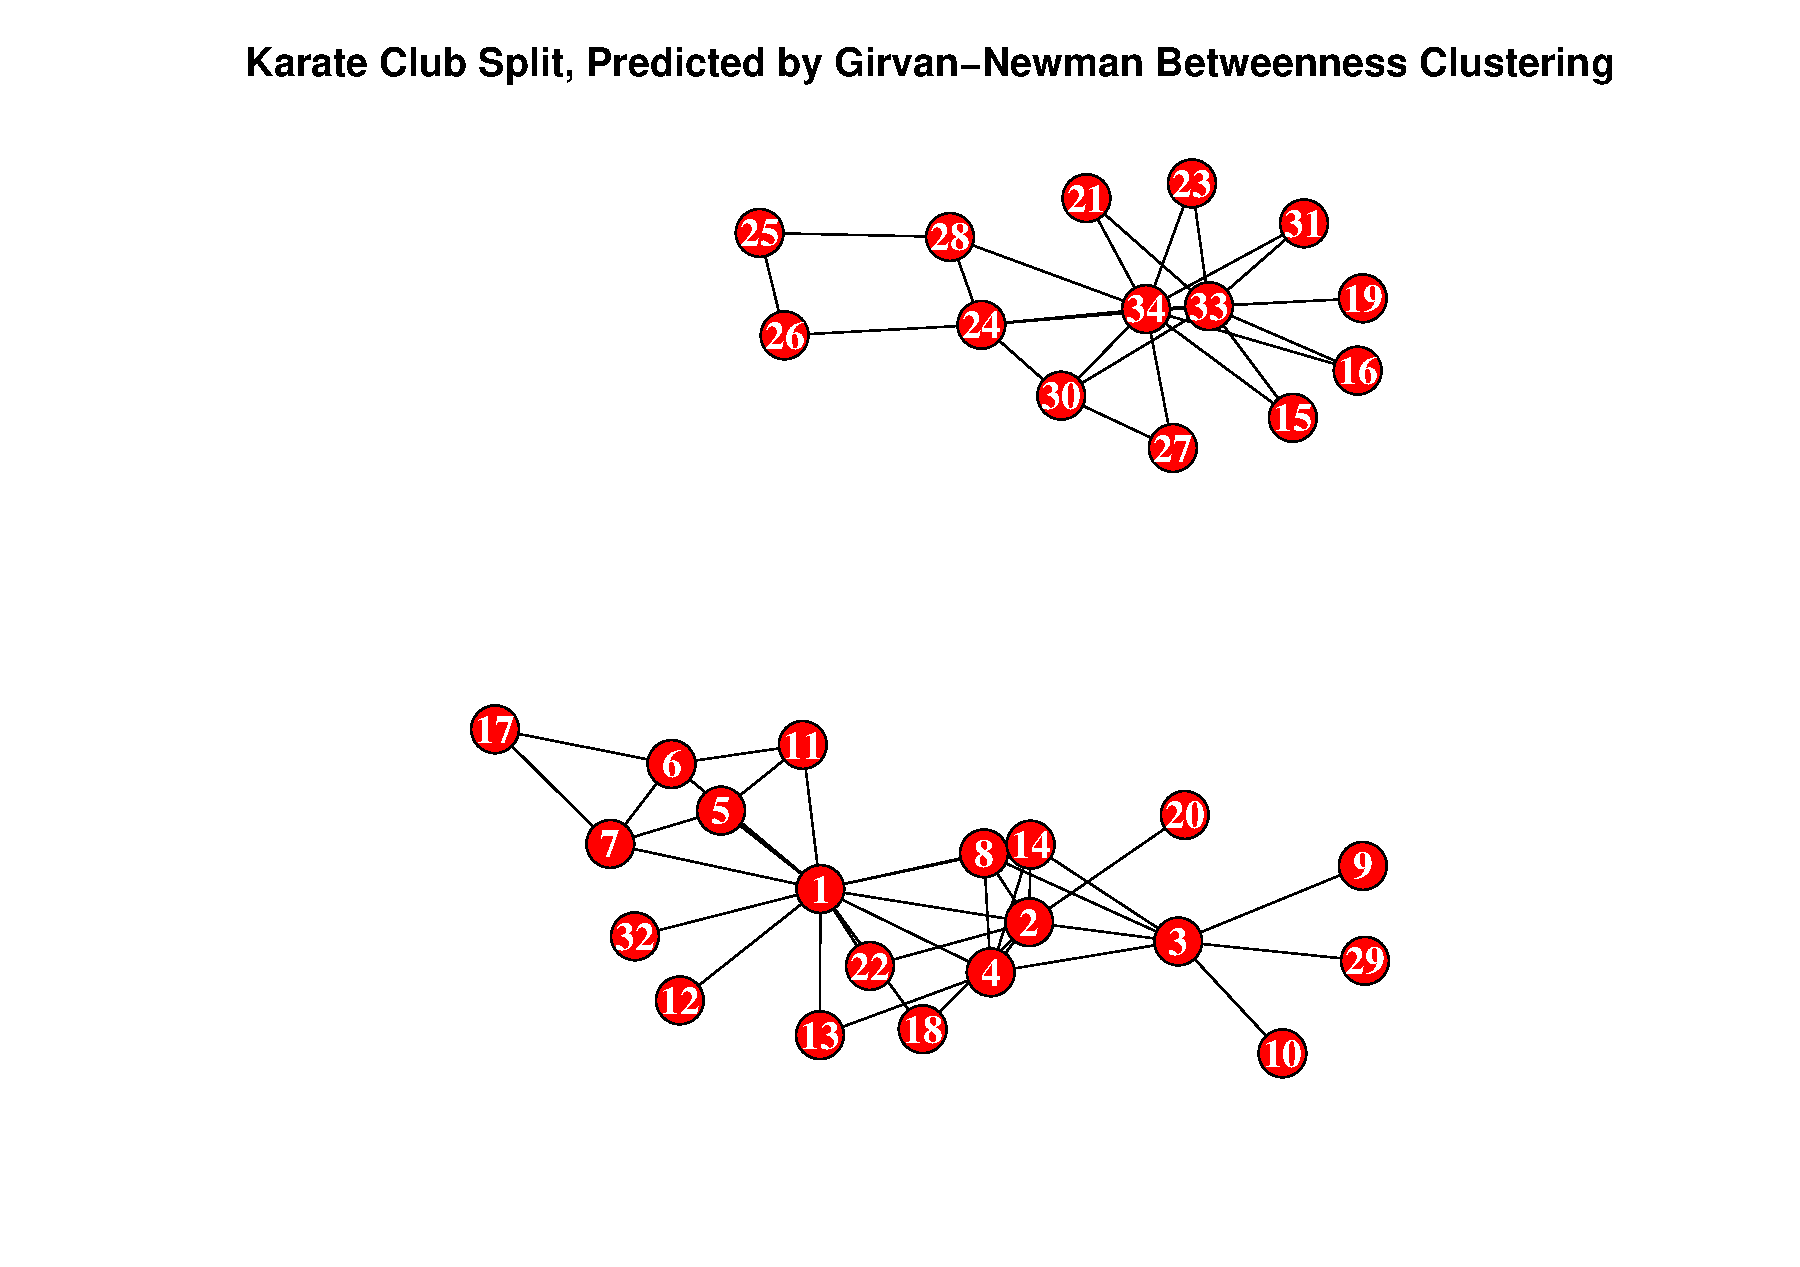
\includegraphics[scale=0.5]{club-after.pdf}
\caption{Karate Club Graph Split Predicted by Girvan \& Newman Betweenness Clustering}
\label{fig:club-after}
\end{figure}

\clearpage
\lstinputlisting[language=R,frame=single,caption={R program for Girvan \& Newman Betweenness Clustering shown in Figures \ref{fig:club-before} and \ref{fig:club-after}},label=lst:q1codeR,captionpos=b,numbers=left,showspaces=false,showstringspaces=false,basicstyle=\footnotesize]{R-code/community-functions.R}

\newpage


\section*{2}

\subsection*{Question}

2.  We know the group split in two different groups.  Suppose the
disagreements in the group were more nuanced -- what would the clubs
look like if they split into groups of 3, 4, and 5?


\subsection*{Answer}

The same R script shown in Listing \ref{lst:q1codeR} was run to produce Figures \ref{fig:club-3-split}, \ref{fig:club-4-split}, and \ref{fig:club-5-split}.  The value of the variable \emph{threshold} on line $7$ was changed to $3$, $4$, or $5$ as needed to create the split.  In all cases, ``Mr. Hi'' and ``John A.'' held on to the largest groups even after the graph was split into $5$ groups.

\begin{figure}[h]
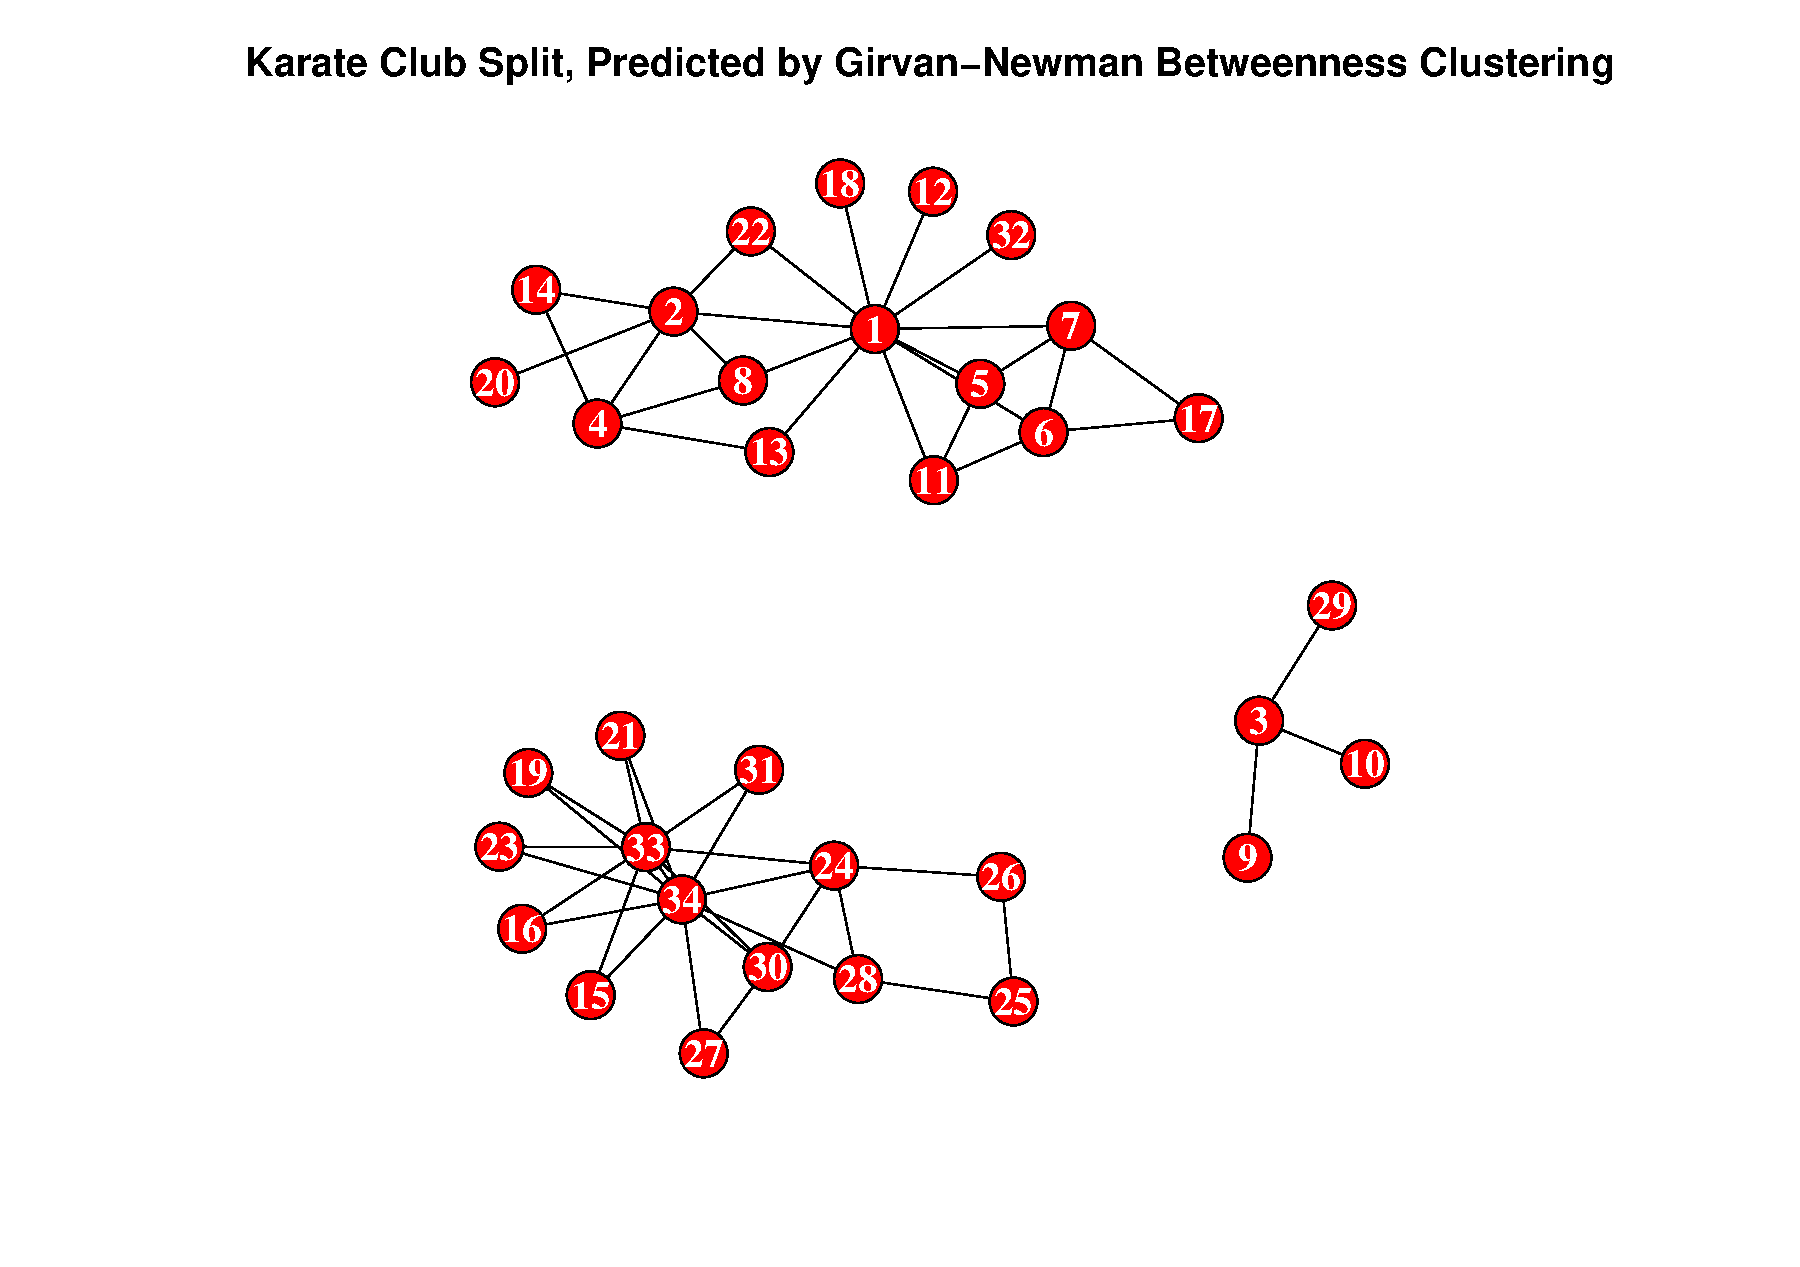
\includegraphics[scale=0.5]{group-of-3.pdf}
\caption{Karate Club Graph Split Into 3 Groups Predicted by Girvan \& Newman Betweenness Clustering}
\label{fig:club-3-split}
\end{figure}

\begin{figure}[h]
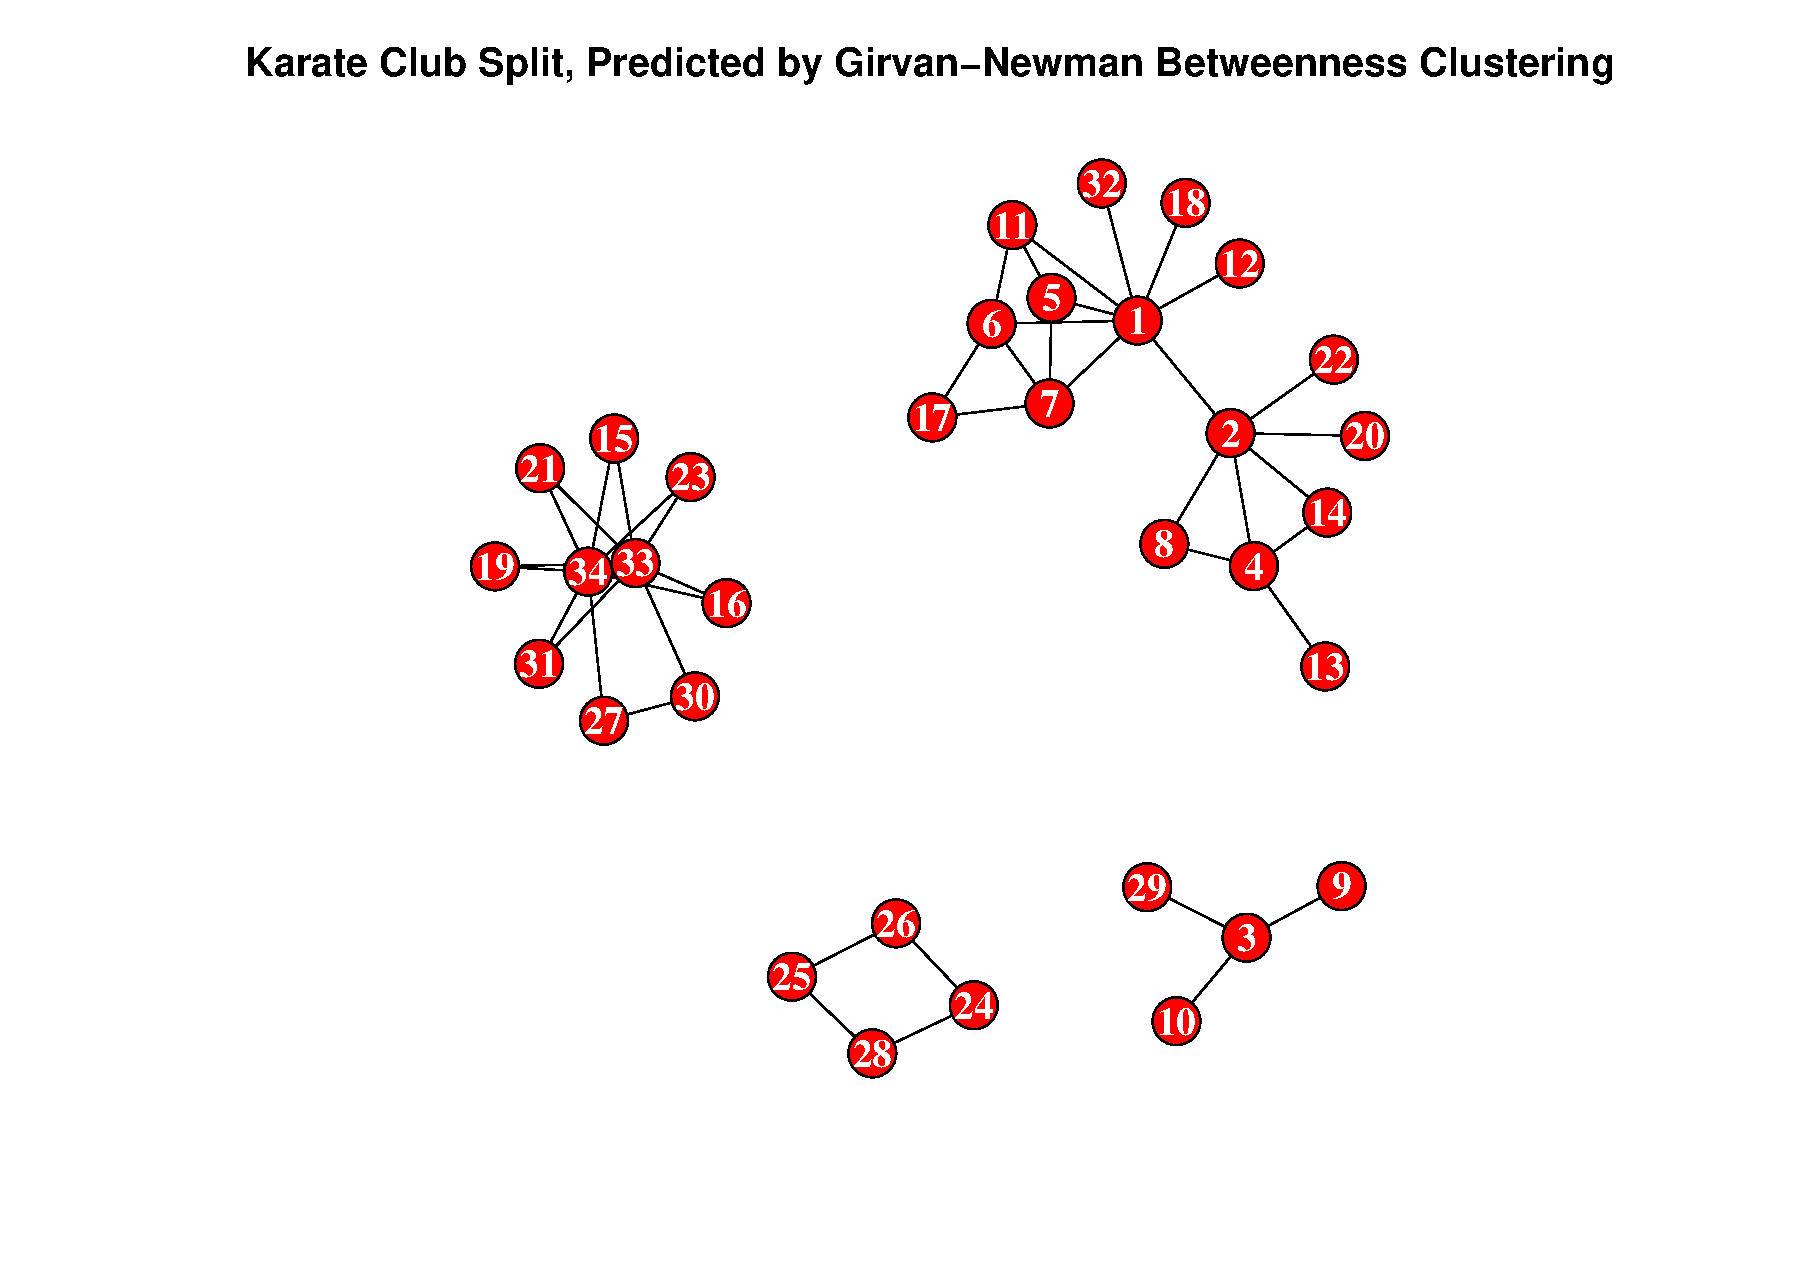
\includegraphics[scale=0.5]{group-of-4.pdf}
\caption{Karate Club Graph Split Into 4 Groups Predicted by Girvan \& Newman Betweenness Clustering}
\label{fig:club-4-split}
\end{figure}

\begin{figure}[h]
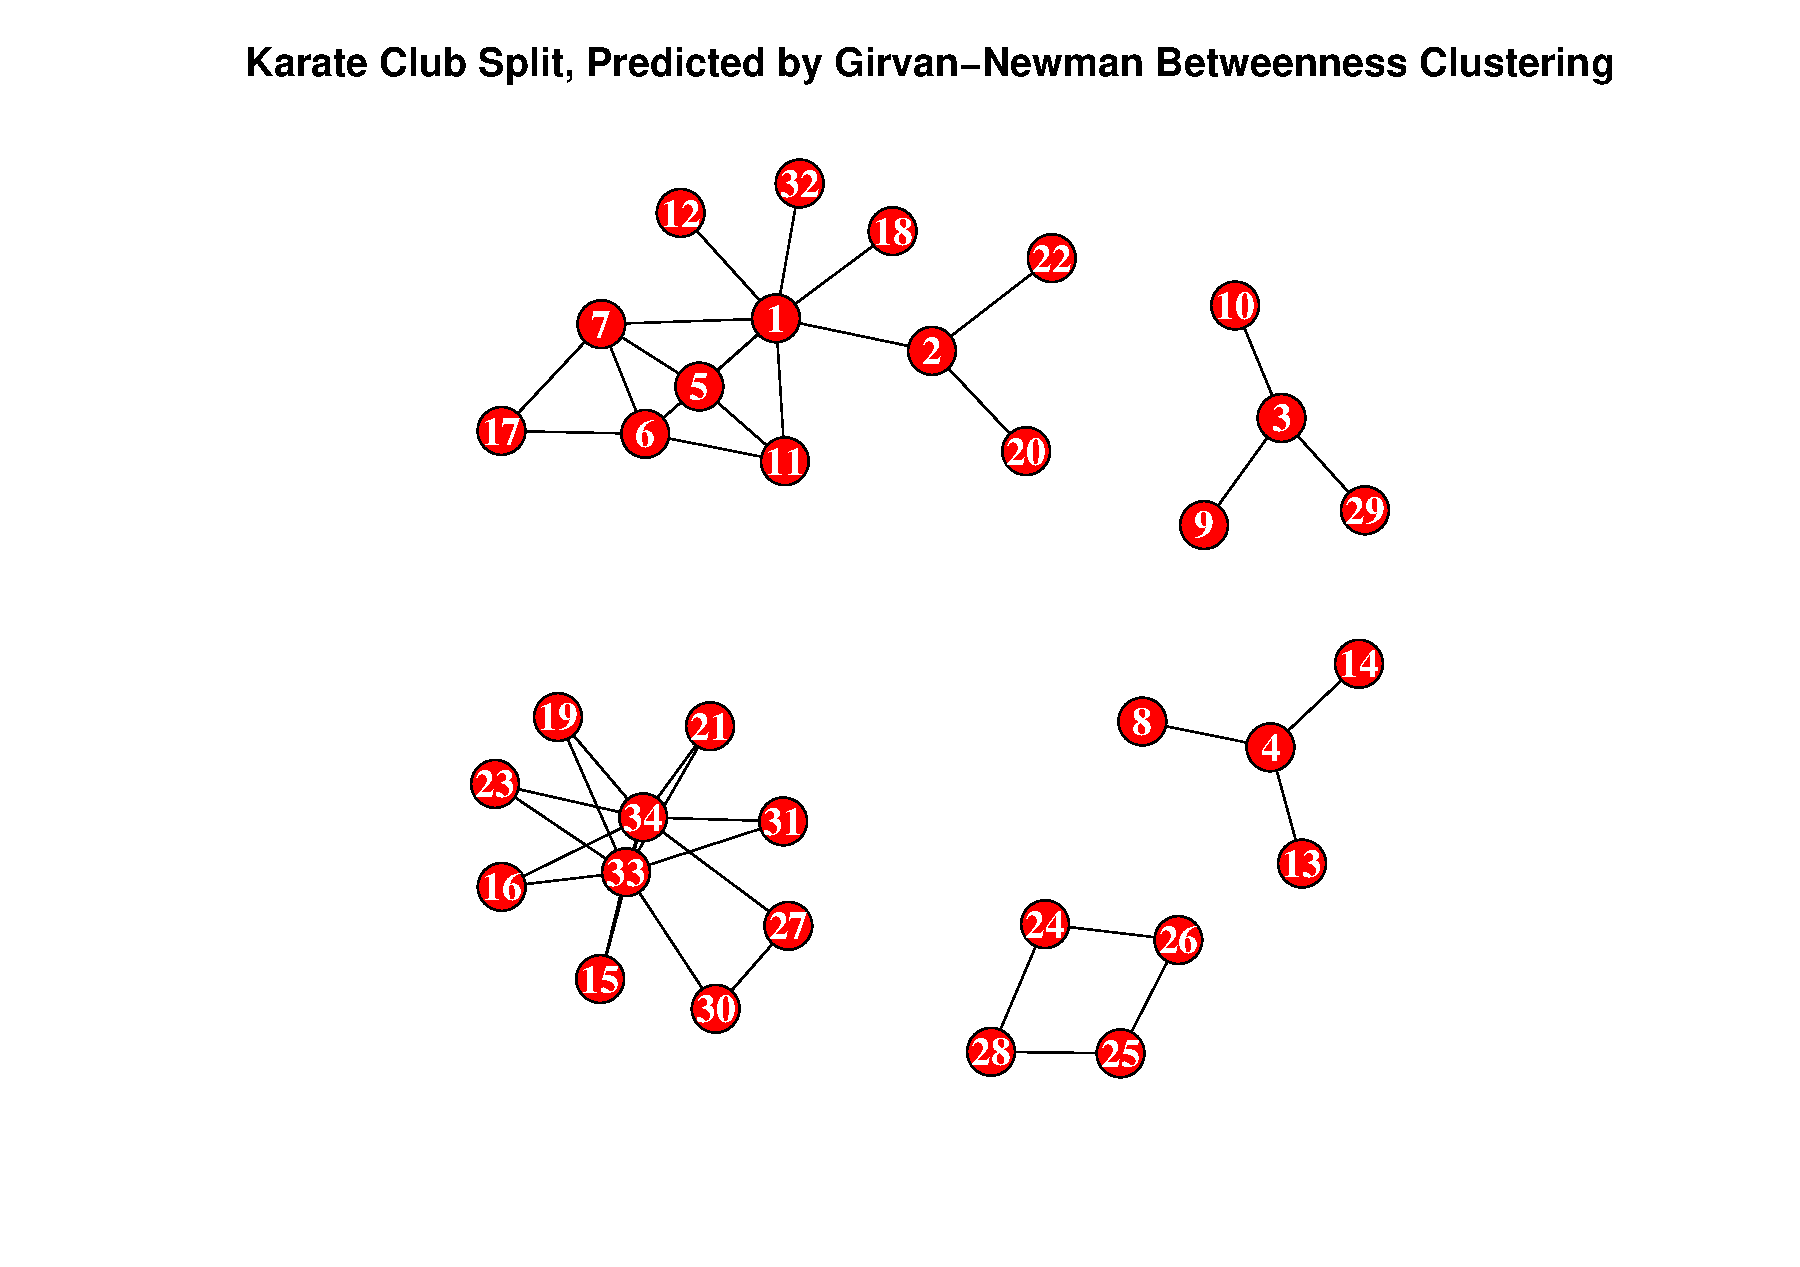
\includegraphics[scale=0.5]{group-of-5.pdf}
\caption{Karate Club Graph Split Into 5 Groups Predicted by Girvan \& Newman Betweenness Clustering}
\label{fig:club-5-split}
\end{figure}


\clearpage
\bibliographystyle{acm}
\bibliography{references}

\end{document}